% soctepmlate
% Author: Vojtěch Boček
% Edit by: Jaroslav Páral
% Version: 2018-02-12
% Source code: https://github.com/RoboticsBrno/soctemplate/
% Base on: http://www.jcmm.cz/cz/sablona-soc.html
% License: CC BY 4.0

\documentclass{template/socthesis}

\usepackage{subcaption}
\usepackage{amsmath}
\usepackage{enumitem}

\addbibresource{text.bib}

\titlecz{Modulární stavba soutěžních robotů}
\titleen{Modular construction of robots}
\author{Tomáš Rohlínek}
\field{10} % Obory SOČ: 1 - 18 (http://www.soc.cz/obory-soc/)
\school{Střední průmyslová škola a Vyšší odborná škola Brno, Sokolská, příspěvková organizace}
\mentor{mgr. Miroslav Burda}
\mentorstatement{mgr. Miroslava Burdy}

% Změňte, pokud se liší
%\region{Jihomoravský}
\placefooter{Brno 2020}

\begin{document}
	\maketitle
	
	\makecopyrightstatement{V~Brně}
	
	\makethanks{Děkuji svému vedoucímu mgr. Miroslavu Burdovi za pomoc, podnětné připomínky a hlavně nekonečnou trpělivost.}
	
	\pagestyle{empty}
	
	\section*{Anotace}
	Cílem této práce je vytvořit sadu univerzálních senzorů pro soutěžní roboty, přičemž jejich instalace, využívání a případná tvorba nových, byla co uživatelsky nejpřívětivější.
	
	\subsection*{Klíčová slova}
	robotika; senzory; komunikace; modulární konstrukce
	
	\vspace{20mm}
	
	\section*{Annotation}
	The goal of this work is to create a pack of sensors for competetive robots, while their installation, usage and creation, is as user friendly, as possible. 
	
	\subsection*{Keywords}
	robotics; sensors; communication; modular construction
	
	\newpage
	\pagestyle{plain}
	
	\tableofcontents % vysází obsah
	
	%%% Začátek práce
	\setcounter{figure}{0}
	\setcounter{table}{0}
	\newpage
	
	%%% Úvod
	\chapter*{Úvod}
\addcontentsline{toc}{chapter}{Úvod} % přidá položku úvod do obsahu
%odsazení od vrchu moc velké
V~poslední době se robotické soutěže těší stále většímu zájmu jak veřejnosti, tak konstruktérů.
Mezi v~česku známé robotické soutěže patří například Pražský robotický den\cite{Prague-robotic-day} a Robotiáda\cite{Robotiada}.
Senzory dosahují různé kvality a používají různé komunikační protokoly a sběrnice, což může být problémem pro začínající konstruktéry, kteří se díky nejednotné nabídce musí starat o~věci jako duplicitní adresy na sběrnici, kolize dvou knihoven řídících jednu sběrnici a hardwarové problémy dané sběrnice.

Cílem této práce je těmto začínajícím konstruktérům poskytnou nástroj, který většinu problémů se senzorikou vyřeší za ně, pro pokročilejší konstruktéry pak nabízí úsporu času.
Tito konstruktéři nemusí již senzory, které se neustále opakují, stavět, zapojovat a programovat vždy znovu, ale dostanou do rukou téměř plug-n-play řešení.


\newpage
	
	%%% Jak psát
	\chapter{Běžně používané sběrnice}
Sběrnice dávají jednotlivým modulům možnost vzájemné komunikace.
Často dochází k~záměně pojmu sběrnice a protokol, což je pochopitelné, neboť se mohu v~různých mírách překrývat.
Sběrnicí většinou rozumíme hardwarovou složku komunikace, ta definuje například počet vodičů, napěťové úrovně na těchto vodičích, atd.
Protokolem pak rozumíme formát dat posílaných po sběrnicích.
V~oboru amatérské stavby robotů se v~praxi používá několik sběrnic a protokolů pro získávání dat:
\begin{itemize}
	\item I$^{2}$C
	\item UART
	      \begin{itemize}
		      \item RS-232
		      \item RS-485
	      \end{itemize}
	\item SPI
	\item 1-Wire
	\item Nesběrnicová komunikace
\end{itemize}

\section{I$^{2}$C}
Snad nejpoužívanější sběrnice a protokol zároveň je I$^{2}$C \cite{nxp:UM10204},
také známá jako Inter-Intergrated Circuit\footnote{ Protože je značka I$^{2}$C chráněna, použili ostatní výrobci název TWI, jedná se o~prakticky stejnou sběrnici, pouze pod jiným názvem.}.
Tato sběrnice byla vyvinuta firmou Philips primárně pro připojení periferií, které nevyžadovaly vysoké komunikační rychlosti.
Sběrnice podporuje jak multi-master, tak multi-slave.
Běžná rychlost je 100~kbit/s, ve Fast modu je 400~kbit/s. Novější revize pak umožňují až 5 Mbit/s, s~touto verzí však nemusí být kompatibilní starší zařízení.
I$^{2}$C používá 7-bitovou adresu, což teoreticky znamená, že je na každé sběrnici možno provozovat až 127 zařízení, prakticky je toto číslo značně nižší.
I$^{2}$C využívá TTL.
Maximální délka sběrnice je 1 metr na 100~kBd, sběrnice však nebyla designovaná na provoz po kabelu, jak je zvyklá ji používat většina amatérských nadšenců.

\begin{table}[h]
	
	\centering
	\begin{tabular}{|l|l|l|l|l|} \hline
		Maximální počet zařízení      & 127              \\ \hline
		Maximální délka               & 1~metr           \\ \hline
		Běžná rychlost                & 100~kbit/s        \\ \hline
		Maximální teoretická rychlost & 5~Mbit/s          \\ \hline
		Minimální počet vodičů        & 3~(SDA, SCL, GND) \\ \hline
	\end{tabular}
	\caption{Shrnutí hlavních parametrů I$^{2}$C}
\end{table}



\section{UART}
Další hojně používanou sběrnicí je UART, mezi amatérskou komunitou známá též jako sériová linka.
UART ve skutečnosti není sběrnice jako taková, jedná se spíše o~něco mezi sběrnicí a protokolem.
UART definuje pouze posílaná data (0 a 1), nikoli však způsob jejich posílání či napěťové úrovně sběrnice.
O~to se starají právě jednotlivé implementace\footnote{I přesto se dá UART používat sám o~sobě na TTL (Transistor-Transistor-Logic), v~tom případě je definice napěťových úrovní ponechána jednotlivým zařízením, což může způsobit vzájemnou nekompatibilitu.}.
Nejběžněji používané implementace UARTu jsou:
\subsection{RS-232} % (fold)
RS-232 \cite{RS-232} je implementace UART.
Používá napěťové úrovně +5~V~až +15~V~pro logickou 1 a --5~V~až --15~V   pro~logickou 0, toto platí pro vysílací část.
Přijímací část přidává dvouvoltovou hysterezi kvůli rušení, což znamená +3~V~až +15~V~pro logickou 1 a --3~V~až --15~V~pro logickou 0.
RS-232 potřebuje společnou GND.
\begin{table}[h]
	
	\centering
	\begin{tabular}{|l|l|l|l|l|} \hline
		Maximální počet zařízení      & 2              \\ \hline
		Běžná rychlost                & 115200~baud/9600~baud        \\ \hline
		Maximální teoretická rychlost & 10~Mbit/s       \\ \hline
		Minimální počet vodičů        & 3~(Tx, Rx, GND) \\ \hline
	\end{tabular}
	\caption{Shrnutí hlavních parametrů RS-232}
\end{table}
% subsection RS-232 (end)
\subsection{RS-485}\label{RS-485} % (fold)
RS-485 \cite{RS-485} je další implementace UARTu.
Nepoužívá ale napěťové úrovně oproti společné GND, nýbrž využívá rozdílu napětí na linkách A~a B, ten musí být alespoň 200~mV.
To způsobuje několik věcí:
\begin{itemize}
	\item Pokud vedou obě linky podél sebe, nejlépe jsou-li kroucené, je prakticky nemožné komunikaci zarušit, což je v~prostředí motorů na robotu značná výhoda\footnote{Zároveň to výrazně zvyšuje maximální možnou délku linky, při nižších rychlostech až na 1200~m. Doporučení: rychlost [baud] * vzdálenost [m] $<$ +/- 10$^{8}$.}.  
	\item Není potřeba společná GND.
	\item Pro plný duplexní mód (jedna linka na vysílání a jedna na přijímání) je potřeba dvojnásobný počet vodičů, tedy 4.
\end{itemize}
V~závislosti na použitém převodníku z~UART na RS-485 může být počet zařízení na sběrnici 32 nebo až 128.
\begin{table}[h]
	
	\centering
	\begin{tabular}{|l|l|l|l|l|} \hline
		Maximální počet zařízení      & 32/128              \\ \hline
		Běžná rychlost                & 115200~baud/9600~baud        \\ \hline
		Minimální počet vodičů        & 2 (A, B) \\ \hline
		Maximální vzdálenost		  & 1200~m \\ \hline
	\end{tabular}
	\caption{Shrnutí hlavních parametrů RS-485}
\end{table}
% subsection RS-485 (end)

\section{SPI}
SPI \cite{nxp:AN2847}, neboli Serial Peripherial Interface, je dvoukanálová synchronní multi-slave\footnote{Na sběrnici je naráz připojen pouze jeden master (řídící jednotka) a typem sběrnice omezené množství slave (řízených) zařízení.} sběrnice.
Pro komunikaci využívá 4 vodiče:
\begin{itemize}
		\item MOSI (Master Output Slave Input) -- výstup z~master a vstup do slave
		\item MISO (Master Input Slave Output) -- výstup ze slave a vstup do master
		\item SCK -- hodinový signál
		\item SS (Slave Select) -- tímto pinem nastavujeme, který slave je momentálně aktivní
\end{itemize}
Na straně masteru může pak díky tomu být počet použitých pinů větší (3~+~počet slave zařízení).

Další možná konfigurace je tzv. Daisy-chain, kdy je  MOSI masteru připojeno na MOSI prvního slave zařízení a MISO prvního slave zařízení je připojeno na MOSI dalšího slave zařízení, až MISO posledního slave zařízení je připojeno na MISO masteru.
Tato konfigurace poskytuje snížení počtu vodičů, zároveň ale snižuje i komunikační rychlost, protože informace od prvního slave zařízení musí obejít celý kruh, než se dostanou zpět k~master zařízení.

Nespornou výhodou SPI je její rychlost.
Maximální rychlost není definovaná, aplikace běžně jdou až přes 10~Mb/s.
Nevýhodou může být velký počet vodičů, př použití standartního zapojení.


\section{1-Wire}
1-Wire \cite{one-wire} je sběrnice (a protokol zároveň), která, jak již její název napovídá, potřebuje pouze jeden vodič.
K~tomu potřebuje ještě společnou GND, ale i tak to jsou pouze 2~vodiče, které obsáhnou napájení i komunikaci\footnote{Sběrnici je možno provozovat i na třílinkovém módu.}.
Této typologie se využívá třeba u~kontaktních přístupových čipů.
Sběrnice je také poměrně známá pro svůj CRC součet, který umožňuje kontrolu odeslaných dat.
1-Wire je kompatibilní s~TTL.
Každé zařízení na sběrnici má unikátní neměnnou adresu.


\section{Nesběrnicová komunikace}
Některé senzory nepotřebují posílat velké množství dat, a proto může být lepší nepoužít sběrnici. 
Příkladem takového senzoru může být třeba obyčejné tlačítko.
Některé senzory zmíněné v~další kapitole také používájí tento způsob předávání dat.
Hlavní problém tohoto řešení je především náročnost na čas procesoru a počet vodičů.


	
	%%% Několik formálních pravidel
	\chapter{Běžně používané senzory na soutežních robotech}

Každý robot potřebuje mít způsob interakce s~okolím.
Tuto interakci zajišťují právě senzory.
Naprostá většina amatérských týmů nemá prostor ani pros\-třed\-ky vytvářet vlastní senzory.
Používání průmyslových senzorů je znemožňováno několika faktory.
Zřejmě nejzásadnějším je cena, dále pak jejich velikost a hmotnost způsobená jejich robustností a kvalitou provedení.
Týmy jsou tedy nuceny používat hotové senzorové moduly, o~nichž často nevědí, jaké komponenty obsahují a jak fungují.
Senzory se dají rozdělit do několika kategorií:
\begin{itemize}
    \item Senzory vzdálenosti
        \begin{itemize}
            \item Ultrazvukové senzory
            \item IR senzory
            \item Lidar/Radar/Sonar
        \end{itemize}
    \item Senzory barvy
        \begin{itemize}
            \item Black-white senzory
            \item RGB senzory
            \item Kamery
        \end{itemize}
    \item Senzory pohybu
        \begin{itemize}
            \item Akcelerometry
            \item Gyroskopy
            \item Enkodéry
            \item Kompasy
        \end{itemize}
    \item Komplexní polohové senzory
\end{itemize}

\section{Senzory vzdálenosti}

Senzory pro zjišťování vzdálenosti dodávájí robotovi poměrně primitivním způsobem schopnost přibližně určit svou polohu na základě vzdáleností od okolních objektů.
Podmínky pro jejich použití jsou však často velmi specifické a nedají se proto samy o~sobě použít pro přesnější lokalizaci.

\subsection{Ultrazvukové senzory}

Asi nejpoužívanějšími senzory vzdálenosti jsou senzory ultrazvukové.
Ty fungují na principu vyslání ultrazvuového pulzu a čekání na jeho návrat.

Nejběžněji používaný z~nich je HC-SR04~\cite{hc-sr04}. 
Ten obsahuje ultrazvukový přijímač a vysílač, spolu s~dodatečnou elektronikou.
Má čtyři vývody: 
\begin{table}[h]
	
	\centering
	\begin{tabular}{|l|l|l|l|l|} \hline
		GND & společná zem/-   \\ \hline
		VCC/5~V~& napájení 5~V/+  \\ \hline
		Echo & Návrat měřené vzdálenosti   \\ \hline
		Trig & Spouštění meření \\ \hline
    \end{tabular}
    \caption{Vývody HC-SR04}
\end{table}

Měření započne posláním logické 1 na pin Trig po dobu alespoň 10~$\mathrm{\mu}$s.
Poté, co Trig opět přepneme na logickou 0, vyšle senzor 8 40-ti kHz pulzů, zárověň nastaví na pinu Echo logickou 1.
Po přijetí odraženého ultrazvukového signálu je na pinu Echo opět nastavena logická 0.
Mikrokontroleru poté pouze zbýva měřit, jak dlouho byla na pinu Echo logická 1, tento čas pak dosadí do rovnice:
% \begin{center}
%     % \begin{equation}
%     %     $\mathrm{vzdálenost=(naměřený čas*rychlost zvuku)}/2$
%     %     \label{eq: Vzdálenost při měření ultrazvukovým senzorem}
%     % \end{equation}
    
    
% \end{center} 
Senzor je schopen měřit vzdálenosti od 2~cm do 4~m, dělá to při 15$^{\circ}$ úhlu.
Senzor má nevalnou přesnost (+/-~2~cm).
Největší úskalí při používaní tohoto senzoru nastává, pokud je na hřišti více robotů, nebo nesynchronizovaných senzorů, kdy se senzory mohou navzájem rušit.
Další problém může vyvstat při používaní pouze jednoho mikroprocesoru a několika ultrazvukových senzorů, kdy čas potřebný na změření všech senzorů přesáhne únosnou mez, čímž se zásadně prodlouží reakční čas robota.
Tento problém se řeší použitím sekundárního procesoru pro obsloužení měření.


\subsection{IR senzory}
Infračervené senzory fungují vesměs na stejném principu jako ty ultrazvukové, pouze ultrazvukové pulzy jsou nahrazeny infračerveným paprskem.
To s~sebou nese oproti ultrazvuku své výhody i nevýhody.
Hlavní výhodou oproti ultrazvuku je menší pravděpodobnost zarušení ambientním signálem, pokud senzor používá modulovaný signál pro měření. 
Nevýhodou je, že stejně jako ultrazvukové senzory mohou být i infračervené senzory přehlceny, v~tomto případě ale spíše silným ambientním zdrojem, například sluncem, než ostat\-ní\-mi senzory.

Nejpoužívanější IR senzor vzdálenosti je FC-51 \cite{fc-51}, který má oproti HC-SR04 výrazně větší měřící úhlel 35$^{\circ}$ a výrazně menší rozsah měřitelných vzdáleností, konkrétně 2~cm až 30~cm.
Na rozdíl od HC-SR04, který měří plynule na celém rozsahu, měří FC-51 pouze přiblížení pod nastavenou mez, podle toho vrací na výstupu 0 a 1.
Hranice přiblížení je nastavitelná pomocí potenciometru nacházejícím se přímo na senzoru.


\subsection{Lidar/Radar/Sonar}
Tato zařízení obsahují běžné senzory vzdálenosti a pouze přidají možnost pohybu těchto senzorů. 
Místo jednosměrného měření pak vytvaří v~podstatě mapu prostoru.
Lidar používá k~měření laserový, většinou IR, paprsek.
Radar používá rádiové vlny, které mohou částečně pronikat materiály, což umožňuje \uv{vidět} skrz zdi.
Sonar používá k~měření zvukové vlny, což je s~výhodou využíváno hlavně pod vodou, kde se tyto vlny velmi dobře šíří.
Bohužel zatím neexistuje spolehlivá a levná iterace těchto senzorů, která by se dala použít na soutěžních robotech.

\section{Senzory barvy}
Senzory barvy jsou použitelné pouze v~některých soutěžních disciplínách.
Dávají našemu robotovi možnost zjišťovat barvu herních objektů a podložky, což může pomoci jak s~orientací, tak s~plněním herních úkolů.

\subsection{Black-white senzory}
Tyto senzory využívají světelný zdroj, zpravidla IR nebo bílý, v~kombinaci s~plynulým světelným senzorem citlivým na vlnovou délku světla zdroje.
Každá látka v~závislosti na své barvě pohlcuje a odráží světlo jinak, nám poté zbývá pouze změřit, kolik světla se odrazilo.
Senzory tedy defakto neměří, jestli je povrch černý nebo bílý, ale spíše jestli je světlý či tmavý.
Existuje obrovské množství iterací tohoto senzoru -- některé plynulé, jiné digitální s~nastavitelnou hranicí překlopení.
B-W senzory se nejčastěji používají v~soutěžích jako line follower\footnote{Soutěž, ve které se robot pokouší co nejrychleji projet dráhu vyznačenou nejčastěji černou čárou na podložce. V~poslední době se do cesty přidávají také překážky, kterým se robot musí vyhnout.}, kde není potřeba kompletní RGB detekce.

\subsection{RGB senzory}
RGB senzory kombinují více B-W senzorů do jednoho celku.
Existují dvě možnosti, jak toho dosáhnout. 

První možnost používá jeden bílý zdroj světla a více senzorů citlivých na specifické vlnové délky, zpravidla 3 senzory pro RGB, občas se také přidává IR a UV.
Všechny senzory přitom mohou měřit naráz.

Druhá možnost používá jeden senzor se širokým spektrem a více zdrojů světla s~různými barvami vyzařovaného světla, opět se nejčastěji používá RGB a případně se k~tomu přidává UV a IR.
Tato možnost má o~něco pomalejší měření oproti první metodě, neboť zdroje světla se musí ve svícení střídat.

\subsection{Kamery}
Zvláštní případem barevných senzorů jsou kamery.
Ty však vyžadují v~závislosti na způsobu použití poměrně velký výpočetní výkon.
To řeší použití samostatného procesoru pro zpracování obrazu, jako to dělá třeba populární Pixy\cite{pixy}\footnote{Nebo můžeme použít aplikaci ve smartphonu, ty pro podobné aplikace mají výpočetního výkonu dostatek. Některé novější by mohly dokonce spustit nějaké Deep learning algoritmy pro zpracování obrazu.}.

Kamery poskytují výhodu hlavně co se zorného pole a vzdálenosti od povrchu týká, nemusí totiž být na rozdíl od dvou předchozích připevněny do několika milimetrů od měřeného povrchu.

\section{Pohybové senzory} 
Senzory pohybu poskytují robotu schopnost určit, jak se v~prostoru pohybuje, některé přímo a některé nepřímo.
Všechny však vyžadují nějaký způsob přepočtu.
Tyto senzory neposkytují vždy přesné údaje, což není způsobeno přímo senzory, ale spíše typem a nedokonalostmi pohybu, který mají měřit.
Polohové senzory, vyjma enkodérů, se zpravidla nepoužívají samostatně, ale v~celcích.
Například běžně používaný senzor mpu-6050 \cite{mpu6050} spojuje dohromady akcelerometr a gyroskop, zárověň má možnost připojit přímo na sebe kompas, což umožňuje vytvořit 9-osý systém.


\subsection{Akcelerometry}
Akcelerometry měří lineární zrychlení.
Ve větším provedení se jedná o~závaží na pružině, která je na druhé straně uchycená k~pouzdru. 
Lineární zrychlení zjístíme změřením a přepočtem změny délky pružiny, neboli o~kolik se pružina zmáčkla/roztáhla, aby uvedla závaží do stejné rychlosti jako má pouzdro.
V~menším provedení se využívá piezoelektrického jevu pro měření.
Senzor může měnit hodnoty v~závislosti na teplotě, to je potřeba buď kompenzovat ve výpočtu, nebo zanedbat -- v~případě nepotřeby superpřesných údajů \cite{accel}.

\subsection{Gyroskopy}
Gyroskopy měří úhlovou rychlost, případně úhel náklonu.
Ve velkém provedení se jedná o~setrvačník připevněný k~pouzdru způsobem, který umožňuje rotaci v~měřených osách.
Rotující setrvačník si zachová nezávisle na pohybu pouzdra svůj počáteční náklon.
Díky tomu máme referenční objekt, od kterého můžeme měřit náklon.
V~menším provedení se používá několik principů, jeden z~nich je Disk Resonator Gyroscope, který využívá pro měření Coriolisovy síly.
Pro měření všech 3 os je potřeba více gyroskopů
\cite{gyro}
\cite{gyro-2}.

\subsection{Enkodéry}
Enkodéry slouží k~převádění mechanického pohybu kol na elektronický signál.
Enkodéry se dají rozdělit na ty, co se používají přímo na pohonu a na vlečné enkodéry.

Enkodéry umístěny na pohonu zabírají méně místa než ty vlečné. 
Na druhou stranu, pokud proklouzne kolo, či část převodu, nemají to tyto senzory jak zjistit.

Vlečné enkodéry mohou mít problém se změnou směru pohybu.
Nejsou však ovlivněny možným proklouznutím hnacího kola, to proto, že měří pohyb relativně k~podložce, na rozdíl od těch umístěných na pohonu, které měří pohyb relativně k~robotovi.


\subsection{Kompasy}
Stejně jako běžné kompasy se elektronické kompasy používají k~zjištění natočení robota v~magnetickém poli Země.

\section{Komplexní polohové senzory}
Když potřebujeme přesné měření polohy, nestačí nám samostatné senzory, musíme vytvořit větší komplexní celek.
Příklad takového systému je Global Positioning System, nebo jeho alternativy jako GLONASS a Galileo.
Tento systém využívá sadu satelitů, které neustále vysílají svou pozici společně s~časem odeslání zprávy.
Pokud přijme přijímač data od alespoň 4 satelitů, může pomocí těchto zpráv triangulovat svoji polohu s~vysokou přesností.

Další lokalizační systém používá HTC Vive \cite{htc}, sada pro vyrtuální realitu, využívající Steam VR \cite{steam} tracking.
Ta je pomocí 2 majáčků schopna s~přesností na milimetr určit polohu senzoru v~prostoru.
Nástroje pro tvorbu vlastních přijímačů jsou navíc volně dostupné, což z~tohoto systému činí perfektní způsob lokalizace objektů v~trojdimenzionálním prostoru.
Jediná problematická věc je cena majáčků (199\$), které je potřeba koupit, neboť zatím nebyly uvolněny podklady, na základě nichž by bylo možné vytvořit vlastní iteraci majáčků.



	
	
	%%% Nikdy to nebude naprosto dokonalé
	\chapter{Volba parametrů}
\section{Sběrnice}
Pro svou práci jsem zvolil sběrnici RS-485.
Hlavní důvody pro toto rozhodnutí jsou:
\begin{itemize}
    \item Odolnost proti rušení
    \item Počet zařízení
    \item Malý počet vodičů -- 2
    \item Celková robustnost
\end{itemize}

\section{Protokol}
Rozhodl jsem se nevyužít již existující protokol, nýbrž sepsat protokol vlastní, tak, aby byl jednoduchý a přizpůsobitelný mým potřebám. 
\section{Zpracované senzory}
Senzory plánované pro implementaci do této sady zahrnují:
\begin{itemize}
    \item Všesměrový ultrazvukový senzor
    \item Sběrač\footnote{Viz kapitola \ref{Sberac}} pro ultrazvukové senzory HC-SR04 
    \item Senzor pro Line follower
    \item RGB senzor
    
\end{itemize}
Kromě senzorů mají být součástí sady i další jednotky:
\begin{itemize}
    \item Battery pack -- inteligentní baterie
    \item Co-processing unit -- přídavná výpočetní jednotka
    \item Rozbočovač -- v~případě potřeby možnost rozšířit sběrnici o~více zařízení
    \item Buffer -- kombinace co-processing unit a rozbočovače
\end{itemize}
\section{Procesory}

Rozhodl jsem se použít pro všechny senzory i řídící jednotku procesory z~řady ESP32.
Některé z~důvodů:
\begin{itemize}
    \item Built--in podpora pro RS-485 přímo v~UART driveru ESP32
    \item Built--in podpora CRC\footnote{Cyklický redundantní součet. Kontrolní prvek využívaný ke kontrole správnosti přijatých dat, běžně používaný mimo jiné na sběrnici 1-Wire, nebo protokolu Modbus.}
    \item Kompletní podpora C++v14 a STL na rozdíl od běžně používaných ATMEGA čipů, používaných například v Arduino deskách
    \item Kompatibilita se spoustou rozhraní a sběrnic -- může sloužit jako převodník mezi ostatními sběrnicemi a Janus protocol/RS485
    \item OTA -- možnost nahrávání programu přes internet\footnote{Snaha o~co nejjednodušší dodatečné opravy systému, kdy si senzory budou samy schopny dostahovat nejnovější firmware, a na obalu nebudou muset být vyvedené programovací konektory.}
    \item WiFi a Bluetooth -- v~případě nutnosti bezdrátové komunikace
    \item Kompatibilita s~Arduino\footnote{Přestože samotný kód protokolu nevyžaduje Arduino a je postaven čistě na ESP-IDF, je Arduino prostředí pro mnoho začátečníků přijemnější pro práci než většina ostatních. Jeho jednoduchost a kompatibilita s~jinými čipy však může zásadně limitovat jeho funkce, proto není obsluha protokolu napsaná právě v~něm.}
\end{itemize}
	
	%%% Typografické a jazykové zásady
	\chapter{Janus protocol}
Janus protocol je snaha o vytvoření co uživatelsky nejpřivětivějšího a zárveň robustního protokolu.
Tento protokol je postavený z velké části na Avakar protokolu.
Přidává k němu adresaci zpráv a kontrolní byte.

\section{Základní specifikace}
\begin{itemize}
    \item Multi-slave
    \item Podpora zpráv různých délek - při zachování minimální délky
    \item Až 254 zařízení (limitováno RS-485 na 32/128 zařízení - bez použití rozbočovačů)
    \item Jednoduché přidání dalšího senzoru do již sestaveného systému
    \item Nutnost restartu celého systém při nahrazování senzorů, nebo změně řídící jednotky
\end{itemize}
	
	%%% Slovo Romana
	\chapter{Slovo Romana}
Titulní strana v~takové podobě, v~jaké se vám dostala, je navzdory veškeré projevené snaze velice chatrná a proto vám radím příliš nezasahovat do její stavby, neboť by to mohlo zcela rozhodit pozice všech objektů.
Primární snahou bylo dosáhnout její netečnosti vůči příliš dlouhým jménům (doc.
RNDr.
Jana Šťastně Vdaná, Ph.D.), názvům práce a názvům škol.

I~v~sekci Prohlášení zkuste držet svého kreativního ducha na uzdě, abyste jej vzápětí uplatnili v~celém následujícím textu.
Struktura textu by měla být zhruba následující:

\begin{enumerate}
\item[$\bullet$] úvod
\item teorie
\item metodika
\item výsledky
\item diskuze
\item[$\bullet$] závěr
\end{enumerate}
nicméně není pevně daná a spoustě prací sluší i tematičtější způsoby dělení informací.

\section{Plovoucí objekty}
Všechna čest Microsoftu za postupnou konverzi Wordu z~textového procesoru v~sázecím software.
Jedna z~mnoha vlastností nových verzí je možnost přidání titulku k~plovoucímu objektu, jako bývá obrázek či tabulka.

\begin{figure}[h]
  	\centering
 	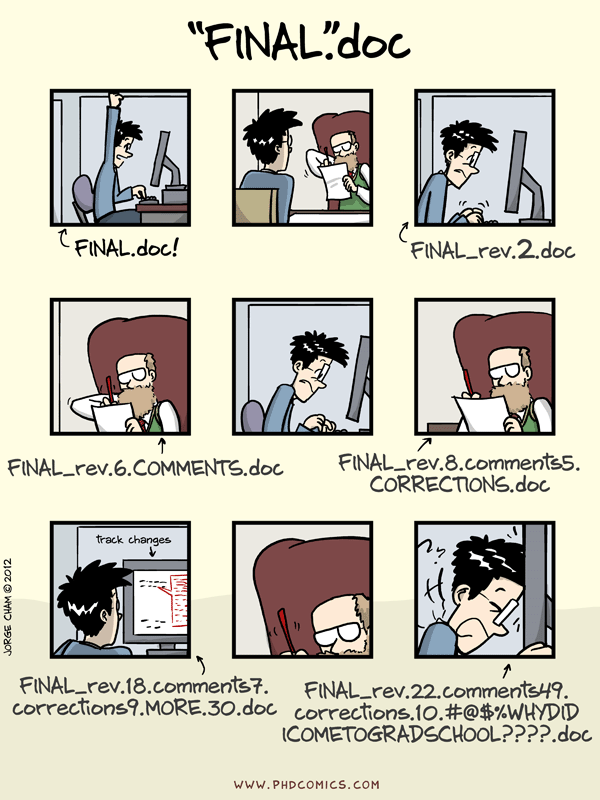
\includegraphics[width=200px]{img/final_doc.png}
 	\caption{Vás to nejspíše čeká taky.}
\end{figure}

\begin{table}[h]
  \centering
    \begin{tabular}{|l|l|}
    \hline
    Jednoduchá & tabulka \\ \hline
    o~& ničem \\
    \hline
    \end{tabular}
  \caption{Jak vidno, čísluje se separátně}
\end{table}

\begin{listedequation}[h]
$$L = - \frac{1}{4}F_{{\mu}v}F^{{\mu}v} + i \overline{\psi} \psi + \psi_i y_i \psi_j \phi + hc + |D_\mu\phi|^2 - V(\phi)$$
\caption{To je ale rovnice!}
\label{eq:hrnekeq}
\end{listedequation}

Vkládání popisků k~obrázkům a tabulkám lze zařídit poměrně snadno a intuitivně tlačítkem „Vložit titulek“ na kartě \It{Reference}.
U~rovnic se bohužel tento způsob uplatňuje jen velmi těžko, klasické vpravo zarovnané (1.1) lze pouze vykouzlit.
(Nápověda Microsoftu radí použít VBA makro, přívrženci Visual Basicu tedy nebudou mít problém.
Obávám se ale, že takových moc nebude.)

Využijte funkci „Vložit seznam obrázků“, která krom seznamu obrázků umí vkládat i seznam tabulek nebo rovnic.
Seznam obrázků v~práci být musí, i kdyby tam byl jen jeden obrázek.
Pro případ nejasnosti upřesňuji, že graf je považován za obrázek.

Co se dá naopak použít skvěle, jsou křížové odkazy.
Klepnutím na tlačítko „Křížový odkaz“ na kartě \It{Reference} mi umožní v~textu odkazovat na právě nějaký z~plovoucích objektů (či kapitolu, sekci, …) Proto nemám potíž zde uvést, že rovnice \autoref{eq:hrnekeq} odpovídá rovnici vyobrazené na hrnku na \autoref{fig:hrnek}, jen s~tím rozdílem, že na hrnku není formulována zcela správně.

\begin{figure}[h]
  	\centering
 	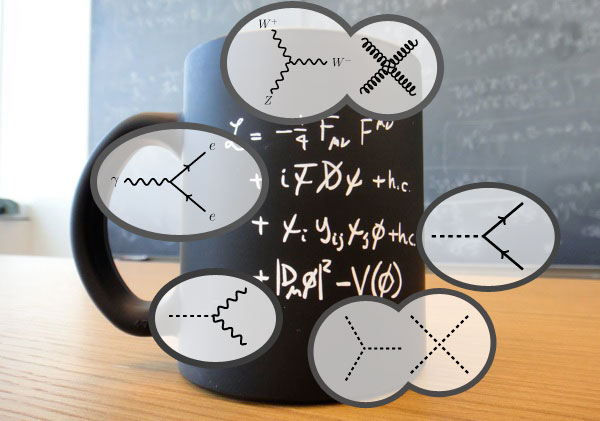
\includegraphics[width=\textwidth]{img/hrnek.jpg}
 	\caption{Hrneček ze Švýcarska}
 	\label{fig:hrnek}
\end{figure}

\section{Bibliografie}
Citovat je důležité (kruciální) a neméně důležité je citovat správně, a to v~ČR podle normy ČSN ISO 690 a ČSN ISO 690-2.
Důvod, proč ji tak mnoho lidí nedělá, je takový: Jedná se o~pěkně otravnou činnost\cite{citovani}.
To se však dá značně eliminovat použitím vhodného softwaru na správu a export citací.
Jaké máme možnosti?

Přímo českou normou se již dlouhou dobu zabývá projekt Citace.com umožňující zdarma získat toliko potřebné bibliografické záznamy.
Proces zkomfortňování šel až tak daleko, že si (např.) čtenáři registrovaní v~Moravské zemské knihovně (do 19 let vč.
zdarma) mohou nainstalovat do svého Wordu doplněk, který téměř vše zařídí za vás.

Pokud náhodou ještě nemáte a nemůžete mít účet v~Moravské zemské knihovně, nemusíte zoufat, i volně přístupná část nástrojů Citací.com má co nabídnout.
Na webu totiž můžete jednoduše vložit ISBN knihy nebo DOI (\It{Digital object identifier}) článku v~časopise a obratem vám bude vygenerována citace přesně podle normy, kterou můžete jednoduše zkopírovat do Wordu.
Číslování v~textu si však budete muset řešit sami.

Nicméně možnosti nekončí Citacemi.com, existuje celá řada dalších nástrojů (třeba EndNote).
Nebojte se požádat o~pomoc své školitele, sami si nejednou prošli stejným problémem a řešení s~velkou pravděpodobností našli.
Tak proč vynalézat kolo?

\subsection{Užitečné odkazy}
\begin{itemize}
    \item \url{http://www.citace.com}, \url{http://www.mzk.cz/}
	\item \url{http://www.boldis.cz/citace/citace1.pdf}
	\item \url{http://www.boldis.cz/citace/citace2.pdf}
	\item \url{https://sites.google.com/site/novaiso690/}
\end{itemize}

\section{Symboly, zkratky, slovníček}
Zkratky vysvětlujeme již při první zmínce v~textu, při jejich častějším výskytu může být praktické uvést ucelený seznam.
Totéž pak platí pro pojmy, které vysvětlujeme v~poznámce pod čarou\footnote{Poznámku pod čarou vložíme opět z~karty \It{Reference} tlačítkem \It{Vložit pozn.
pod čarou.}}: pokud jich je mnoho, vysázíme je i samostatně jako slovníček pojmů.

\section{Moudra závěrem}
Uvědomte si, že hlavním výstupem vaší roční činnosti nejsou data nebo zařízení, nýbrž právě odborný text, který má komisi SOČ ukázat, jak jste studované problematice porozuměli, jaký je váš vlastní přínos, jestli dokážete verbálně vystihnout vše podstatné a důležité.
\It{Formální a estetickou úpravou práce sdělujete komisi, jak moc vám záleží na tom, aby pro ně bylo čtení vaší práce příjemným či alespoň snesitelným zážitkem.}

Šablona je míněna jen jakýmsi odrazovým můstkem a nebojte, pořád na vás zbylo docela dost práce.
Bohužel víc, než jsem původně zamýšlel, protože sázení ve Wordu stále není žádný med a byla by jistě škoda ochudit vás o~četné nadávky na nesmyslnost jeho chování.
Všem počítačově zdatným jedincům pak doporučuji naučit se sazbu v~LaTeXu, je to dovednost, která se vám nikdy neztratí.

\begin{figure}[h]
  	\centering
 	
\includegraphics[width=\textwidth]{img/pulp.jpg}
 	\caption{Nejste v~tom sami.}
\end{figure}

Na závěr vám už poradím jen jedno: hledejte inspiraci.
Velmi dobře si pamatuji ten pocit, kdy sedíte nad prázdným dokumentem a přemýšlíte, co vlastně do té SOČky patří.
Kde začít? Co ještě zmínit a co už raději vynechat? Přitom máme všichni díky theses.cz na dosah stovky tisíc závěrečných prací starších kolegů z~vysokých škol.
Najděte si svůj vzor a jeďte podle něj, odborné posudky vedoucích a oponentů vám dokonce řeknou, co je správně a co nikoliv.

\vspace{\baselineskip}
\noindent Vědě zdar!

\vspace{\baselineskip}
\noindent \B{Roman Beránek} \\
\url{ischemy@gmail.com}

	
	%%% Slovo Jarka
	\chapter{Slovo Jarka}
Trochu bych nesouhlasil s~Romanem ohledně „hlavního výstupu vaší roční činnosti“ a také se zdroji, odkud je vhodné čerpat inspiraci.

Rád bych tato dvě témata na závěr trochu rozebral a zároveň přidal pár slov o~prezentacích, které by měly tvořit podstatnou část vaší práce.

\section{Hlavní výstup vaší roční činnosti}
U~některých oborů možná platí, že hlavním výstupem vaší roční činnosti nejsou data nebo zařízení, nýbrž právě odborný text.
Ovšem z~vlastní zkušenosti mohu říct, že pokud předvedete funkční výtvor (a to ať už softwarový balík pro vývoj a řízení aplikací s~mikročipy, výukový webový portál, univerzální ovládací pult, nebo regulovatelný napájecí zdroj) budete mít na 90 \% větší úspěch než čistě teoretická práce.

Samozřejmě pokud někdo vyvrátí teorii relativity nebo vymyslí novou a lepší periodickou tabulku prvků, bude mít pravděpodobně lepší pozici než vy.
Proto ale musí být vaše práce co možná nejlepší.

Pokud donesete výrobek, který je inovativní, nadčasový, velmi nápaditý a případně vyrobitelný nebo dokonce komerčně prodatelný, a dokážete ho při prezentaci prodat (o~důležitosti prezentace více informací níže), většina porotců vám promine i formální nedostatky a krátký rozsah práce, protože jste jim to předvedli naživo (minimálně toto platí v~rámci oboru strojírenství, elektra a informatiky a podle mě i fyziky, učebních pomůcek atd.)

Kdybych to vzal do extrému, tak práce, která nemá text, ale je velmi zajímavá pro svůj výrobek (zařízení), může klidně vyhrát celostátní kolo SOČ.
Ovšem když přijdu s~textem, kde tento výrobek dokonale popisuji, ale nedovezu, nepředvedu, neukáži, že je funkční, tak jsem na tom hůř než v~prvním případě.

Toto jsou ovšem specifika spíše techničtějších oborů (s~kterými mám zkušenost) a je možné, že v~přírodních vědách (jako chemie, matika, biologie) má spíše Roman pravdu, ale nejsem si tím úplně jistý.
Zvažte sami~:-)

\section{Kde čerpat inspiraci}
Roman jako inspiraci doporučoval theses.cz, ovšem já bych vás spíše odkázal na archiv SOČ (\url{http://soc.nidm.cz/archiv}) a to ze tří důvodů:

\begin{enumerate}[label=\alph*)]
	\item Uvidíte styl a způsob zpracování úspěšných prací SOČ, které vytvořili studenti ve vašem věku a které se porotcům líbily.
	\item Nemusíte se probírat stovkami tisíc závěrečných prací, ale jednoduše si vyberete váš obor a projdete několik nejlepších prací za posledních pár let.
	\item Styl bakalářských a diplomových prací se od SOČek trochu liší a občas je lepší se držet zaběhnutých pravidel SOČ.
\end{enumerate}
Samozřejmě si můžete projít i několik vysokoškolských prací a třeba v~nich najdete i lepší inspiraci.

Jinak nad samostatným formátováním (či některými detaily) neztrácejte mnoho času, protože vám pravděpodobně schází ještě podstatnější věci.
A~také platí, že co porotce/obor, to jiný názor na některé detaily formátování SOČek :-)

\section{Prezentace}
Sebelepší práce bez dobré prezentace je prakticky k~ničemu.
Porotci v~nižších kolech (okresních i krajských) nemají často čas prostudovat si text práce předem.
Tudíž jej občas vidí poprvé, až když danou práci prezentujete.

Pokud budete mít dobrou prezentaci, ve které svoji práci dobře prodáte – ukážete, co jste dělali, jak jste to dělali, co je vaše práce, ale hlavně co je tak unikátního na vaší práci a proč zrovna vy byste měli vyhrát), tak máte z~poloviny vyhráno.
Prezentace tvoří klidně i polovinu hodnocení vaší práce.
Nebo víc.

Proto je podle mě důležité věnovat minimálně stejné množství času přípravě prezentace jako textu.
Pokud postoupíte do dalšího kola, máte většinou možnost si svou práci vzít a do týdne ji upravit/doladit.
Samozřejmě že pokud budete mít perfektní text hned do prvního kola SOČ, budete mít výhodu vůči ostatním a lepší startovací pozici do dalších kol, ale v~případě nedostatku času (což většinou bývá) je vhodnější rozdělit si čas mezi tvorbu textů, prezentace a případně samostatného výrobku.

Samozřejmě se nebojte inspirovat u~svých kolegů z~minulých let například na serveru YouTuBe (hledejte pod „CP SOČ 2013“ a „SOČ 2013 – Brno – krajské kolo“).

O~prezentacích se toho dá samozřejmě napsat mnoho, ale to si necháme třeba na příště ;-)

\vspace{\baselineskip}
\noindent SOČce zdar!

\vspace{\baselineskip}
\noindent \B{Jarek Páral}\\
\url{paral.jarek@gmail.com}
	
	%%% Slovo Lucie
	\chapter{Ještě slovo Lucie}
Pokud si nebudete jistí typografií nebo pravopisem, konzultujte vynikající Internetovou jazykovou příručku.
Píšou ji autoři z~Ústavu pro jazyk český a mezi množstvím balastu na Internetu jí můžete věřit.
Stačí většinou zadat do Google problémové slovo nebo znak spolu s~heslem „ujc“ a víte, na čem jste.

Doufám, že jsme vám pomohli a zpříjemnili práci na vaší SOČce a že shledáte šablonu přínosnou.
Za podněty a reakce budeme všichni tři rádi.

\vspace{\baselineskip}
\noindent Ať to jde!

\vspace{\baselineskip}
\noindent \B{Lucie Vaškeová} \\
\url{lucie.vaskeova@jcmm.cz}
	
	%%% Závěr
	\newpage
\chapter*{Závěr}
\addcontentsline{toc}{section}{Závěr}

Závěrečná kapitola obsahuje zhodnocení dosažených výsledků se zvlášť vyznačeným vlastním přínosem studenta.
Povinně se zde objeví i zhodnocení z~pohledu dalšího vývoje projektu, student uvede náměty vycházející ze zkušeností s~řešeným projektem a uvede rovněž návaznosti na právě dokončené projekty.

	
	\newpage
	\printbibliography[title=Literatura]
	\addcontentsline{toc}{section}{Literatura}
	
	\listoffigures
	\addcontentsline{toc}{section}{Seznam obrázků}
	
	\listoftables
	\addcontentsline{toc}{section}{Seznam tabulek}
	
	\listoflistedequation
	\addcontentsline{toc}{section}{Seznam rovnic}
	
\end{document}
